\documentclass[11pt,a4paper]{article}
\usepackage[T1]{fontenc}
\usepackage{lmodern}
\usepackage{amsmath,amssymb}
\usepackage{graphicx}
\usepackage{booktabs}
\usepackage[margin=2.3cm]{geometry}
\usepackage{microtype}
\usepackage{xcolor}
\usepackage[section]{placeins}   % keeps floats inside their section
\usepackage[colorlinks=true,linkcolor=blue!50!black,citecolor=blue!50!black,urlcolor=blue!50!black]{hyperref}

\title{Exercise 4\\[2pt]\large Spherical collapse}
\date{}  

\begin{document}
\maketitle

All numbers, tables and figures below are produced by \texttt{notebooks/exercise\_4.ipynb} with the code in \texttt{scripts/exercise\_4.py}, following the smooth-dark-energy, shear-free limit of Pace, Meyer \& Bartelmann~\cite{Pace2017} and the Lecture~8 notes~\cite{Notes}. The background is EdS or flat $\Lambda$CDM, $E^2(a)=\Omega_{m0}a^{-3}+\Omega_{\Lambda0}$ with $\Omega_{\Lambda0}=1-\Omega_{m0}$, with radiation neglected at all epochs.

%------------------------------------------------------------------------------------------------
\section{Formulations A, B, C}

For $N=\ln a$, $A_H = 2+\mathrm{d}\ln H/\mathrm{d}N$, $\vartheta=\nabla_x\cdot\boldsymbol v/(aH)$, $g=1/\delta$,
\begin{align}
\text{A:}\quad & \frac{d^2\delta}{dN^2} = - A_H \frac{d\delta}{dN} + \frac{4}{3} \frac{(\frac{d\delta}{dN})^2}{(1 + \delta)} + \frac{3}{2} \Omega_m\delta (1 + \delta), \label{eq:A}\\
\text{B:}\quad & \frac{\mathrm{d}\delta}{\mathrm{d}N} = -(1+\delta)\,\vartheta, \qquad
\frac{\mathrm{d}\vartheta}{\mathrm{d}N} = -A_H\,\vartheta - \frac{\vartheta^2}{3} - \frac{3}{2}\,\Omega_m\,\delta, \label{eq:B}\\
\text{C:}\quad & \frac{\mathrm{d}g}{\mathrm{d}N} = g\,(1+g)\,\vartheta, \qquad
\frac{\mathrm{d}\vartheta}{\mathrm{d}N} = -A_H\,\vartheta - \frac{\vartheta^2}{3} - \frac{3\,\Omega_m}{2g}. \label{eq:C}
\end{align}
A is integrated as the first-order system $(\delta,\delta_N)$, B and C directly. 

The same state $(N,\delta,\vartheta)$ is written in each formulation's variables ($\delta_N=-(1+\delta)\vartheta$ for A, $g=1/\delta$ for C) and compared through B:
\begin{itemize}
\item A vs B: $\delta_{NN}^A$ vs $-\delta_N\vartheta-(1+\delta)\vartheta_N^B$
\item C vs B: $-\delta^2 g_N^C$ vs $\delta_N^B$, and $\vartheta_N^C$ vs $\vartheta_N^B$
\end{itemize}
Over 20 random states ($N\in[-10,0]$, $\delta\in[10^{-5},10^6]$), the maximum $|x_1/x_2-1|$ is $3.3\times10^{-16}$, $4.4\times10^{-16}$, $2.2\times10^{-16}$ (EdS) and $3.3\times10^{-16}$, $2.2\times10^{-16}$, $2.2\times10^{-16}$ ($\Omega_{m0}=0.3$) for the three comparisons.

%------------------------------------------------------------------------------------------------
\section{Growing-mode initial conditions}

$\delta_{N,i}=f_i\delta_i$ (A), $\vartheta_i=-f_i\delta_i/(1+\delta_i)$ (B, C), $g_i=1/\delta_i$ (C), and for the linear equation $\delta_{L,NN}+A_H\delta_{L,N}-\frac32\Omega_m\delta_L=0$, integrated in parallel with each formulation, $\delta_{L,i}=\delta_i$, $\delta_{L,N,i}=f_i\delta_i$.

$f_i$ is calculated from Exercise 1 at $a_i$ (with ODE evaluated starting at $10^{-3}a_i$).

\begin{table}[htbp]
\centering
\caption{$1-f_i$ at the initial epoch (expected: $f_i=1$ in EdS, and $f_i\to1$ in $\Lambda$CDM for early $a_i$, matter domination).}
\small
\begin{tabular}{c c c c}
\toprule
$\Omega_{m0}$ & $a_i=10^{-3}$ & $a_i=10^{-4}$ & $a_i=10^{-5}$\\
\midrule
1.0 & $-2.2\times10^{-16}$ & $2.2\times10^{-16}$ & $-8.9\times10^{-16}$\\
0.2 & $2.18\times10^{-9}$ & $2.18\times10^{-12}$ & $1.3\times10^{-15}$\\
0.3 & $1.27\times10^{-9}$ & $1.27\times10^{-12}$ & $1.6\times10^{-15}$\\
0.4 & $8.18\times10^{-10}$ & $8.19\times10^{-13}$ & $5.6\times10^{-16}$\\
\bottomrule
\end{tabular}
\end{table}

\begin{figure}[htbp]
\centering
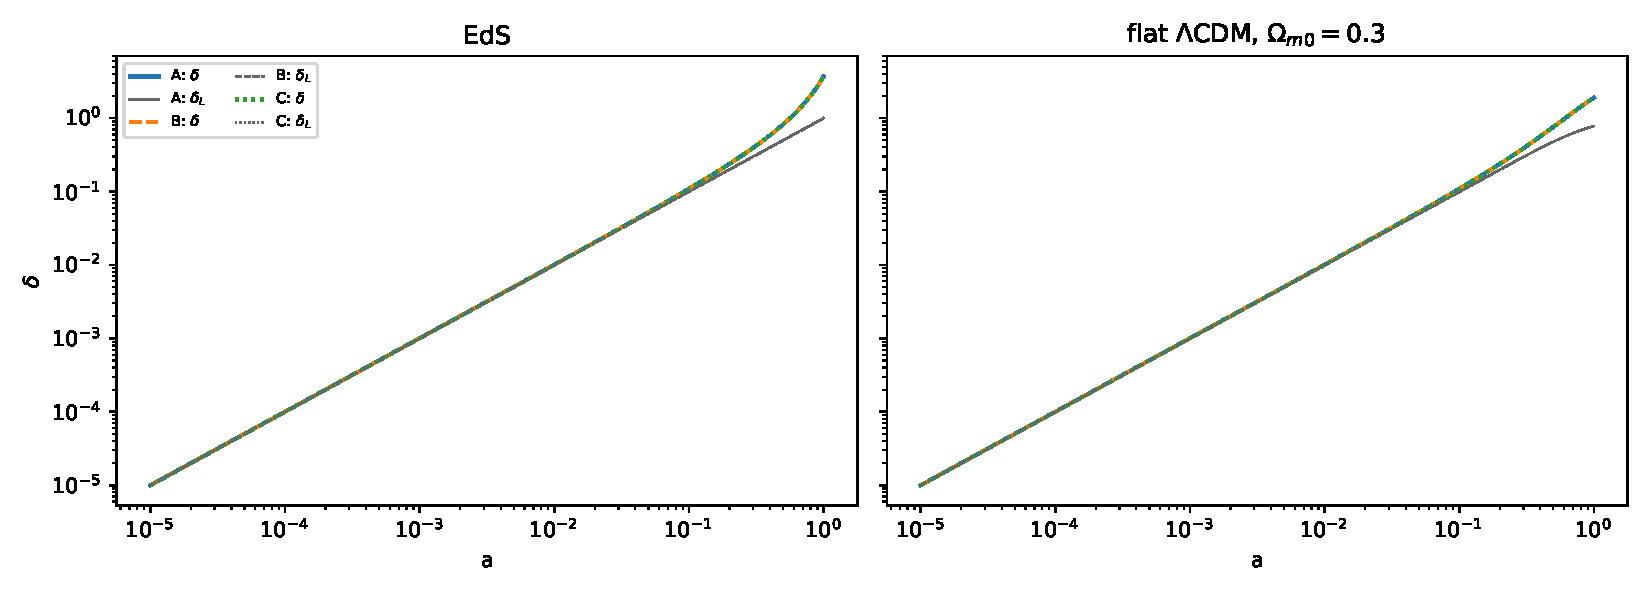
\includegraphics[width=0.95\textwidth]{figures/growing_mode.pdf}
\caption{A, B, C integrated together with their linear counterpart for one trial amplitude, $\delta_i=10^{-5}$ at $a_i=10^{-5}$, from $a_i$ to $a=1$.}
\label{fig:growing}
\end{figure}

%------------------------------------------------------------------------------------------------
\section{Collapse epoch}

For $a_c=(1+z_c)^{-1}$, $\delta_i$ is tuned with \texttt{brentq} until the collapse event ($\delta=\delta_\infty$ for A, B; $g=\epsilon$ for C) happens at $a_c$; then $\delta_c=\delta_L(a_c)$.

Residual: $N_{\rm coll}(\delta_i)-N_c$ (integration to $N_c+0.5$). Bracket: $\pm3\%$ around $1.686\,D(a_i)/D(a_c)$, widened until the sign changes.

For $a_i=10^{-5}$, $\delta_\infty=10^8$ (A, B), $\epsilon=10^{-8}$ (C), ODEs are solved with method DOP853 with \texttt{rtol=1e-10}, \texttt{atol=1e-13}. The collapse event is terminal, so the singular endpoint is never crossed; \texttt{brentq} uses \texttt{xtol}$=10^{-14}\times$guess, \texttt{rtol}$=10^{-14}$.

\begin{table}[htbp]
\centering
\caption{Tuned runs: root-search record and settings ($z_c=0$; $a_i=10^{-5}$, \texttt{rtol=1e-10}, \texttt{atol=1e-13}). Event residual $=\ln(a_{\rm coll}/a_c)$; nfev: right-hand-side evaluations of the tuned run.}
\label{tab:tuned}
\small
\begin{tabular}{c c c c c c c c c}
\toprule
& $\Omega_{m0}$ & threshold & $10^5\,\delta_i$ & $\delta_c$ & bracket $[10^{-5}]$ & iter. & event residual & nfev\\
\midrule
A & 1.0 & $\delta_\infty=10^8$ & 1.6863898 & 1.6863898 & [1.63588, 1.73706] & 6 & $4.5\times10^{-15}$ & 2357\\
B & 1.0 & $\delta_\infty=10^8$ & 1.6863898 & 1.6863898 & [1.63588, 1.73706] & 6 & $-4.2\times10^{-15}$ & 2483\\
C & 1.0 & $\epsilon=10^{-8}$ & 1.6863898 & 1.6863898 & [1.63588, 1.73706] & 6 & $4.5\times10^{-15}$ & 3101\\
A & 0.3 & $\delta_\infty=10^8$ & 2.1508360 & 1.6754604 & [2.10002, 2.22992] & 7 & $-8.3\times10^{-15}$ & 2297\\
B & 0.3 & $\delta_\infty=10^8$ & 2.1508360 & 1.6754604 & [2.10002, 2.22992] & 7 & $1.9\times10^{-15}$ & 2339\\
C & 0.3 & $\epsilon=10^{-8}$ & 2.1508360 & 1.6754604 & [2.10002, 2.22992] & 7 & $-8.0\times10^{-16}$ & 2942\\
\bottomrule
\end{tabular}
\end{table}

\begin{figure}[htbp]
\centering
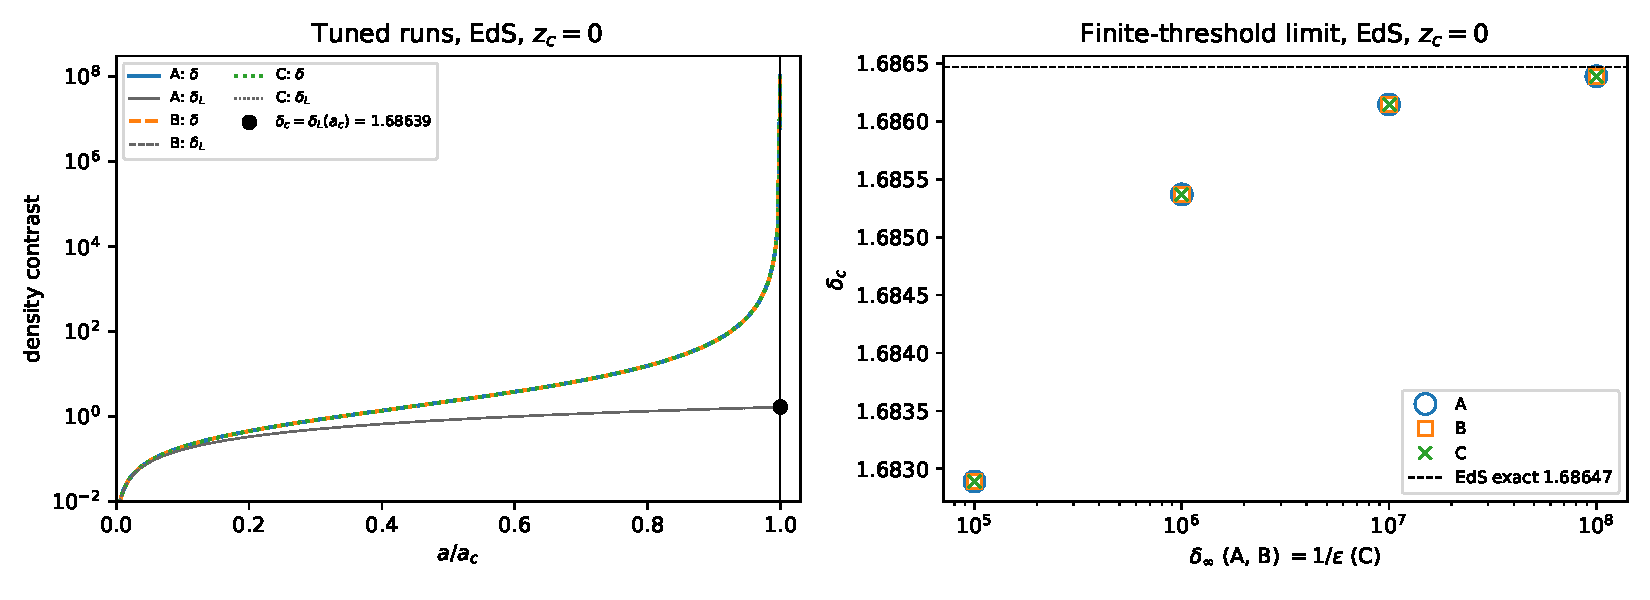
\includegraphics[width=0.95\textwidth]{figures/collapse_epoch.pdf}
\caption{Left: tuned trajectories (EdS, $z_c=0$) up to the collapse event and $\delta_c$ read at $a_c$. Right: $\delta_c$ for each threshold, $\delta_\infty=10^{5\ldots8}$ (A, B) and $\epsilon=1/\delta_\infty$ (C), $\delta_i$ retuned for each.}
\label{fig:collapse}
\end{figure}

The 3 formulations A, B, C reach the threshold at $a_c$ with $|\ln(a_{\rm coll}/a_c)|\lesssim10^{-14}$ and return the same $\delta_c$. As the threshold grows, $\delta_c$ increases.

%------------------------------------------------------------------------------------------------
\section{Turnaround and virial prescription}

\textbf{Turnaround:} $\vartheta(a_{\rm ta}) = -3$, $\quad \zeta_{\rm ta} = 1+\delta(a_{\rm ta})$, with $\vartheta=-\delta_N/(1+\delta)$ in A and $\delta = 1/g$ in C. It is recorded as a non-terminal event on the tuned run (from $\mathrm d\ln R/\mathrm dN=1+\vartheta/3$).

\textbf{Virial prescription}:
\begin{equation}
\lambda_{\rm ta} = \frac{\Omega_\Lambda(a_{\rm ta})}{\Omega_m(a_{\rm ta})\,\zeta_{\rm ta}}, \qquad
4\lambda_{\rm ta}y^3 - 2(1+\lambda_{\rm ta})\,y + 1 = 0, \quad y = \frac{R_{\rm vir}}{R_{\rm ta}} \in (0, 1/2]\ \ (y = 1/2 \text{ in EdS})
\label{eq:cubic}
\end{equation}
\begin{equation}
\Delta_{{\rm vir},m}(a_c) = \zeta_{\rm ta}\left(\frac{a_c}{a_{\rm ta}}\right)^3 y^{-3}, \qquad
\Delta_{{\rm vir},c}(a_c) = \Omega_m(a_c)\,\Delta_{{\rm vir},m}(a_c)
\label{eq:dvir}
\end{equation}
The physical root of eq.~\eqref{eq:cubic} is found with \texttt{brentq} in $(0,1/2]$: $y=0.4999999975$ for $\lambda_{\rm ta}=10^{-8}$, $0.4974876$ for $10^{-2}$, $0.4845798$ for $0.06$, $0.4738957$ for $0.1$, with cubic residuals $\le6\times10^{-16}$.

\begin{table}[htbp]
\centering
\caption{Required outputs of each formulation ($z_c=0$, default settings). A, B and C agree to all digits shown; residuals and costs of each formulation are in Table~\ref{tab:tuned}.}
\label{tab:outputs}
\small
\begin{tabular}{l c c}
\toprule
& EdS & $\Omega_{m0}=0.3$\\
\midrule
tuned $\delta_i$ & $1.6863898\times10^{-5}$ & $2.1508360\times10^{-5}$\\
$a_{\rm ta}$ ($=a_{\rm ta}/a_c$) & 0.6300026 & 0.5614617\\
$\zeta_{\rm ta}$ & 5.5516525 & 6.8373077\\
$\delta_c$ & 1.6863898 & 1.6754604\\
$\lambda_{\rm ta}$ & 0 & 0.0604021\\
$y$ & 0.5 & 0.4844738\\
$\Delta_{{\rm vir},m}$ & 177.61729 & 339.71423\\
$\Delta_{{\rm vir},c}$ & 177.61729 & 101.91427\\
\bottomrule
\end{tabular}
\end{table}

\begin{figure}[htbp]
\centering
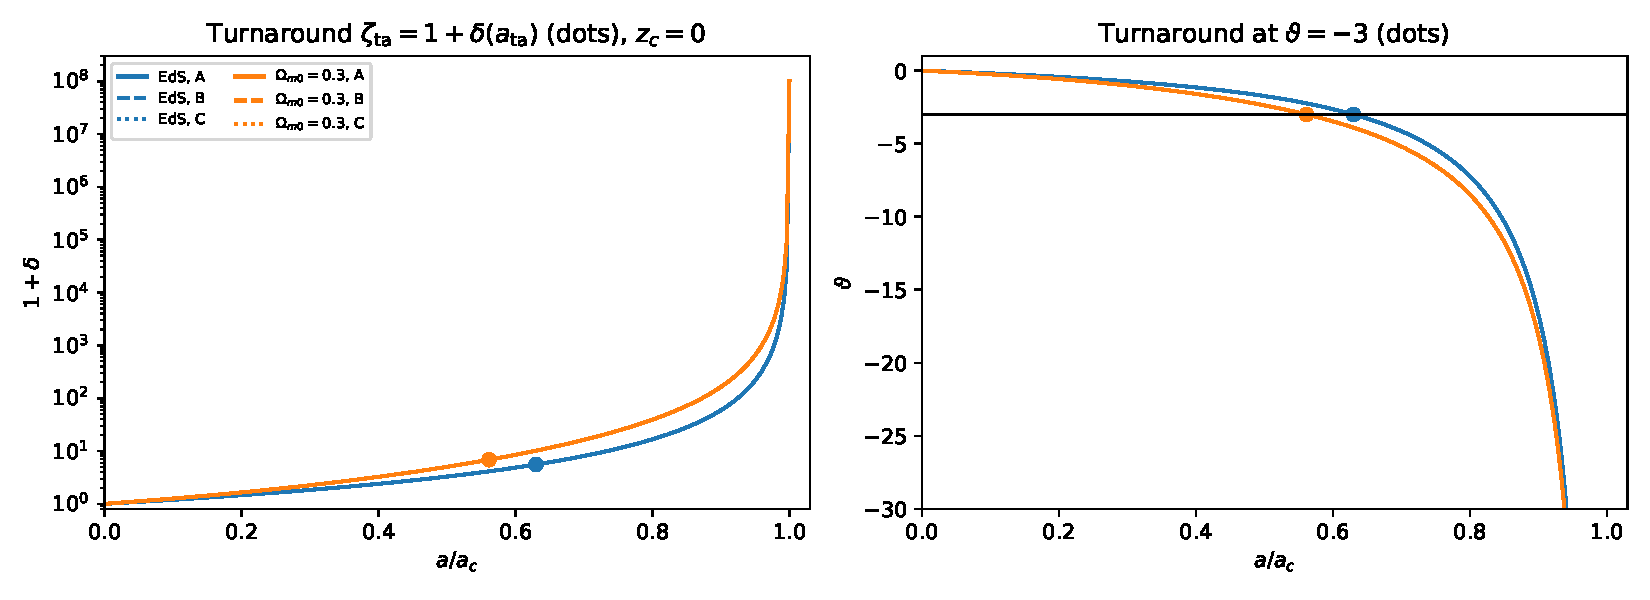
\includegraphics[width=0.95\textwidth]{figures/turnaround.pdf}
\caption{Tuned runs ($z_c=0$) of A, B, C for EdS and $\Omega_{m0}=0.3$. Left: $1+\delta$ with the turnaround $(a_{\rm ta},\zeta_{\rm ta})$ (dots). Right: $\vartheta$, crossing $-3$ at turnaround (dots).}
\label{fig:turnaround}
\end{figure}

A, B, C return same turnaround and virial values.

For EdS: $a_{\rm ta}/a_c=0.6300$, $\zeta_{\rm ta}=5.5517$, $y=1/2$, $\Delta_{{\rm vir},m}=\Delta_{{\rm vir},c}=177.62$

For $\Omega_{m0}=0.3$: $a_{\rm ta}/a_c=0.5615$, $\zeta_{\rm ta}=6.837$, $y=0.4845<1/2$, $\Delta_{{\rm vir},m}=339.7$, $\Delta_{{\rm vir},c}=101.9$

%------------------------------------------------------------------------------------------------
\section{Independent EdS benchmarks}

For $\delta_c=\frac{3}{20}(12\pi)^{2/3}=1.68647$, $a_{\rm ta}/a_c=2^{-2/3}$, $\zeta_{\rm ta}=(3\pi/4)^2$, $\Delta_{{\rm vir},m}=18\pi^2$ at $z_c=0,1,2$.

\begin{table}[htbp]
\centering
\caption{Relative error of each formulation with respect to the exact EdS values (default settings).}
\label{tab:eds}
\small
\begin{tabular}{c c c c c c c}
\toprule
$z_c$ & & $\delta_i$ & $\delta_c$ & $a_{\rm ta}/a_c$ & $\zeta_{\rm ta}$ & $\Delta_{{\rm vir},m}$\\
\midrule
0 & A & $1.69\times10^{-5}$ & $-4.77\times10^{-5}$ & $6.68\times10^{-5}$ & $3.2\times10^{-11}$ & $-2.00\times10^{-4}$\\
  & B & $1.69\times10^{-5}$ & $-4.77\times10^{-5}$ & $6.68\times10^{-5}$ & $5.6\times10^{-12}$ & $-2.00\times10^{-4}$\\
  & C & $1.69\times10^{-5}$ & $-4.77\times10^{-5}$ & $6.68\times10^{-5}$ & $-7.9\times10^{-11}$ & $-2.00\times10^{-4}$\\
1 & A & $3.37\times10^{-5}$ & $-2.86\times10^{-5}$ & $6.68\times10^{-5}$ & $5.1\times10^{-11}$ & $-2.00\times10^{-4}$\\
  & B & $3.37\times10^{-5}$ & $-2.86\times10^{-5}$ & $6.68\times10^{-5}$ & $8.1\times10^{-12}$ & $-2.00\times10^{-4}$\\
  & C & $3.37\times10^{-5}$ & $-2.86\times10^{-5}$ & $6.68\times10^{-5}$ & $-1.4\times10^{-10}$ & $-2.00\times10^{-4}$\\
2 & A & $5.06\times10^{-5}$ & $-9.45\times10^{-6}$ & $6.68\times10^{-5}$ & $-2.3\times10^{-12}$ & $-2.00\times10^{-4}$\\
  & B & $5.06\times10^{-5}$ & $-9.45\times10^{-6}$ & $6.68\times10^{-5}$ & $3.8\times10^{-12}$ & $-2.00\times10^{-4}$\\
  & C & $5.06\times10^{-5}$ & $-9.45\times10^{-6}$ & $6.68\times10^{-5}$ & $1.1\times10^{-10}$ & $-2.00\times10^{-4}$\\
\bottomrule
\end{tabular}
\end{table}

Convergence with the collapse threshold (B, $z_c=0$) is shown in Table~\ref{tab:eds_th}.

\begin{table}[htbp]
\centering
\caption{Relative error with respect to the exact EdS values as a function of the collapse threshold (B, $z_c=0$).}
\label{tab:eds_th}
\small
\begin{tabular}{c c c c c}
\toprule
$\delta_\infty$ & $\delta_c$ & $a_{\rm ta}/a_c$ & $\zeta_{\rm ta}$ & $\Delta_{{\rm vir},m}$\\
\midrule
$10^5$ & $-2.12\times10^{-3}$ & $2.15\times10^{-3}$ & $5.0\times10^{-12}$ & $-6.41\times10^{-3}$\\
$10^6$ & $-6.53\times10^{-4}$ & $6.72\times10^{-4}$ & $5.5\times10^{-12}$ & $-2.01\times10^{-3}$\\
$10^7$ & $-1.92\times10^{-4}$ & $2.12\times10^{-4}$ & $5.6\times10^{-12}$ & $-6.35\times10^{-4}$\\
$10^8$ & $-4.77\times10^{-5}$ & $6.68\times10^{-5}$ & $5.6\times10^{-12}$ & $-2.00\times10^{-4}$\\
\bottomrule
\end{tabular}
\end{table}

The turnaround checks ($a_{\rm ta}/a_c$, $\zeta_{\rm ta}$) and $\Delta_{{\rm vir},m}$ improve together with $\delta_c$ as the threshold grows, so the benchmarks are not recovered by tuning the threshold to $\delta_c$ alone.

%------------------------------------------------------------------------------------------------
\section{Cosmology grid}

$\Omega_{m0}\in\{0.2,0.3,0.4\}$, $\Omega_{\Lambda0}=1-\Omega_{m0}$, $z_c\in\{0,1,2\}$, default settings, formulations A, B, C. The full table of the 27 runs is saved in \texttt{data/lcdm\_grid.csv}.

\begin{table}[htbp]
\centering
\caption{Grid results (formulation C). The cross-formulation spread (max $-$ min over A, B, C) is $\le1.0\times10^{-10}$ in $\delta_c$, $\le7.9\times10^{-11}$ in $a_{\rm ta}/a_c$, $\le2.0\times10^{-9}$ in $\zeta_{\rm ta}$, $\le1.3\times10^{-7}$ in $\Delta_{{\rm vir},m}$ and $\le2.5\times10^{-8}$ in $\Delta_{{\rm vir},c}$ at every grid point.}
\label{tab:grid}
\small
\begin{tabular}{c ccc ccc ccc}
\toprule
& \multicolumn{3}{c}{$\delta_c$} & \multicolumn{3}{c}{$\Delta_{{\rm vir},m}$} & \multicolumn{3}{c}{$\Delta_{{\rm vir},c}$}\\
\cmidrule(lr){2-4}\cmidrule(lr){5-7}\cmidrule(lr){8-10}
$\Omega_{m0}$ & $z_c=0$ & 1 & 2 & 0 & 1 & 2 & 0 & 1 & 2\\
\midrule
0.2 & 1.67161 & 1.68289 & 1.68527 & 440.00 & 216.51 & 189.57 & 88.00 & 144.34 & 165.11\\
0.3 & 1.67546 & 1.68421 & 1.68575 & 339.71 & 200.78 & 184.64 & 101.91 & 155.44 & 169.96\\
0.4 & 1.67817 & 1.68495 & 1.68599 & 286.19 & 192.68 & 182.15 & 114.47 & 162.25 & 172.56\\
\bottomrule
\end{tabular}
\end{table}

\begin{figure}[htbp]
\centering
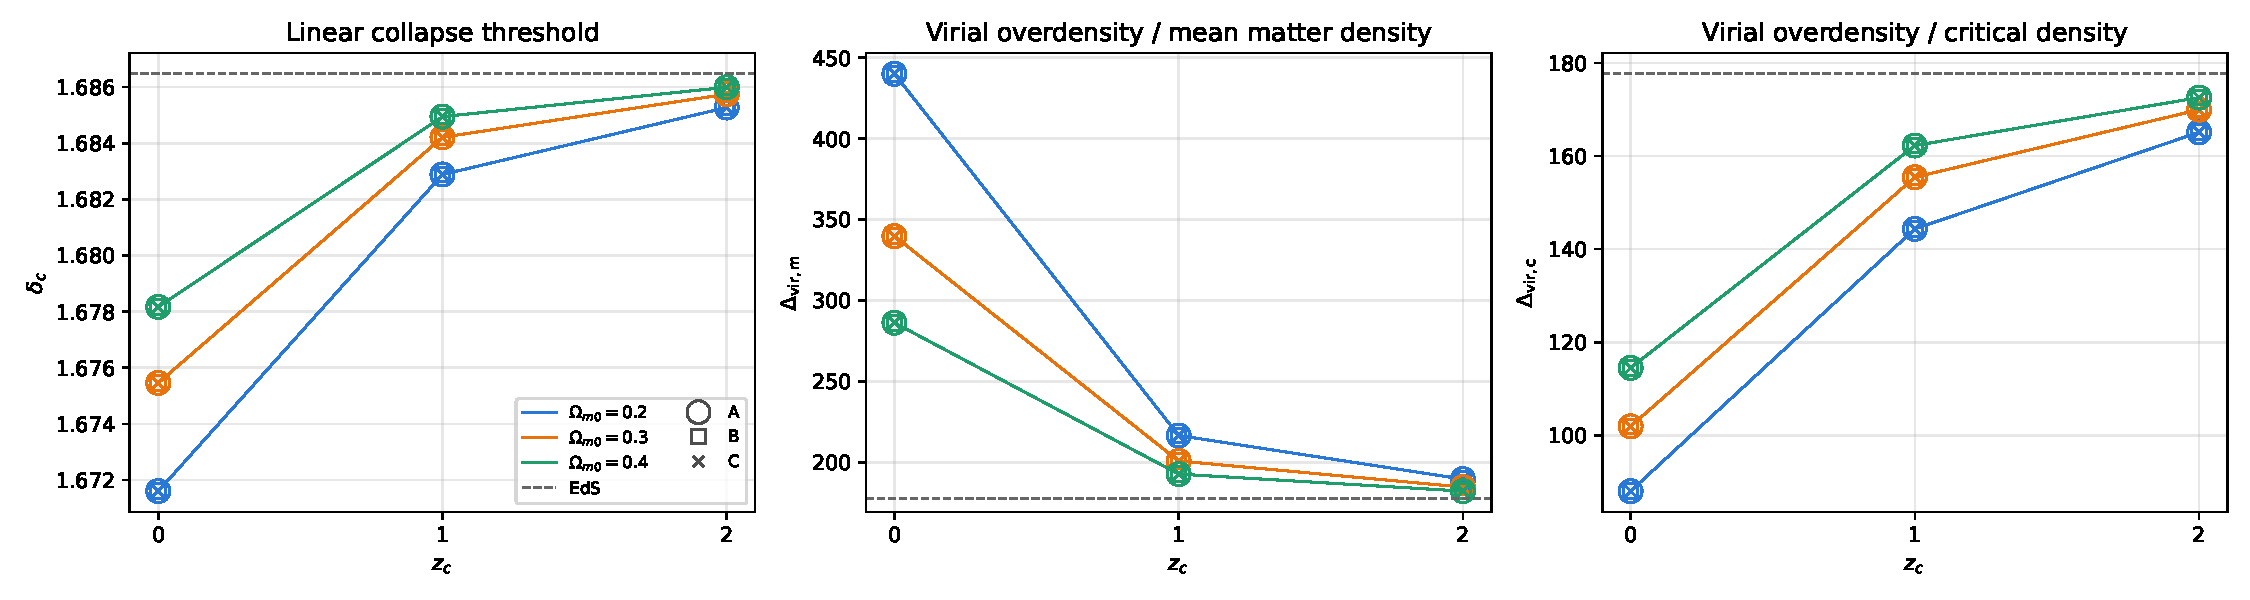
\includegraphics[width=\textwidth]{figures/lcdm_grid.pdf}
\caption{$\delta_c(z_c)$, $\Delta_{{\rm vir},m}(z_c)$ and $\Delta_{{\rm vir},c}(z_c)$ for the flat-$\Lambda$CDM grid; markers: A, B, C; dashed: EdS baselines $1.68647$ and $18\pi^2$.}
\label{fig:grid}
\end{figure}

\begin{table}[htbp]
\centering
\caption{$\delta_c=\delta_i\,D(a_c)/D(a_i)$: initial amplitude and linear growth in $\Lambda$CDM relative to EdS at the same $z_c$ (formulation C).}
\label{tab:growth}
\small
\begin{tabular}{c c c c c}
\toprule
$\Omega_{m0}$ & $z_c$ & growth $\Lambda$CDM / growth EdS & $\delta_i$ $\Lambda$CDM / EdS & $\delta_c$ $\Lambda$CDM / EdS\\
\midrule
0.2 & 0 & 0.70687 & 1.40229 & 0.99123\\
0.2 & 1 & 0.92561 & 1.07810 & 0.99790\\
0.2 & 2 & 0.97479 & 1.02514 & 0.99930\\
0.3 & 0 & 0.77898 & 1.27541 & 0.99352\\
0.3 & 1 & 0.95317 & 1.04776 & 0.99869\\
0.3 & 2 & 0.98489 & 1.01491 & 0.99958\\
0.4 & 0 & 0.83140 & 1.19692 & 0.99513\\
0.4 & 1 & 0.96861 & 1.03150 & 0.99913\\
0.4 & 2 & 0.99015 & 1.00967 & 0.99973\\
\bottomrule
\end{tabular}
\end{table}

\textbf{Growth}: $\delta_c$ is the initial amplitude needed for collapse at $a_c$, evolved in linear theory from $a_i$ to $a_c$. In $\Lambda$CDM, cosmologies with higher values of $\Lambda$ have slower growth of linear perturbations at late times, so for an overdensity to collapse at $a_c$, it needs larger initial amplitudes than in EdS.

\begin{table}[htbp]
\centering
\caption{Factorisation of the virial overdensities relative to EdS: $\Delta_{{\rm vir},m}/18\pi^2 = [\zeta_{\rm ta}/(3\pi/4)^2]\times[(a_c/a_{\rm ta})^3/4]\times[(1/2)/y]^3$, $\Delta_{{\rm vir},c}=\Omega_m(a_c)\Delta_{{\rm vir},m}$ (formulation C).}
\label{tab:factors}
\small
\setlength{\tabcolsep}{4pt}
\begin{tabular}{c c c c c c c c}
\toprule
$\Omega_{m0}$ & $z_c$ & $\Omega_m(a_c)$ & $\dfrac{\zeta_{\rm ta}}{\zeta_{\rm ta}({\rm EdS})}$ & $\dfrac{(a_c/a_{\rm ta})^3}{(a_c/a_{\rm ta})^3({\rm EdS})}$ & $\dfrac{y^{-3}}{y^{-3}({\rm EdS})}$ & $\dfrac{\Delta_{{\rm vir},m}}{\Delta_{{\rm vir},m}({\rm EdS})}$ & $\dfrac{\Delta_{{\rm vir},c}}{\Delta_{{\rm vir},c}({\rm EdS})}$\\
\midrule
0.2 & 0 & 0.200 & 1.342 & 1.618 & 1.141 & 2.477 & 0.495\\
0.2 & 1 & 0.667 & 1.065 & 1.112 & 1.029 & 1.219 & 0.812\\
0.2 & 2 & 0.871 & 1.021 & 1.036 & 1.010 & 1.067 & 0.929\\
0.3 & 0 & 0.300 & 1.232 & 1.412 & 1.099 & 1.912 & 0.574\\
0.3 & 1 & 0.774 & 1.039 & 1.068 & 1.018 & 1.130 & 0.875\\
0.3 & 2 & 0.920 & 1.012 & 1.021 & 1.006 & 1.039 & 0.957\\
0.4 & 0 & 0.400 & 1.165 & 1.290 & 1.072 & 1.611 & 0.644\\
0.4 & 1 & 0.842 & 1.026 & 1.045 & 1.012 & 1.085 & 0.913\\
0.4 & 2 & 0.947 & 1.008 & 1.013 & 1.004 & 1.025 & 0.971\\
\bottomrule
\end{tabular}
\end{table}

\textbf{Turnaround}: the spheres of overdensities reach turnaround when they stop expanding due to their self-gravity. In $\Lambda$CDM, higher values of $\Lambda$ make the background expansion accelerate, which means that overdensities need to reach higher values for turnaround. Indeed, $\zeta_{\rm ta}$ is larger for smaller values of $\Omega_m$. For higher values of $\Lambda$, it also happens earlier in relation to the collapse, which makes $\Delta_{{\rm vir},m}$ increase.

\textbf{Virial prescription}: For a uniform sphere of mass $M$ and radius $R$ in a flat background with matter and a cosmological constant $\Lambda$, the virial prescription is defined based on the assumptions:
\begin{itemize}
\item For the gravitational potential energy of the sphere $U_G = -\dfrac{3GM^2}{5R}$ and the potential energy of the sphere in the $\Lambda$ field $U_\Lambda = -\dfrac{\Lambda M R^2}{10}$, turnaround happens when the sphere is at rest ($K=0$) and $E_{\rm ta} = U_{G,\rm ta} + U_{\Lambda,\rm ta}$
\item It virializes when $2K + U_G - 2U_\Lambda = 0 \;\Rightarrow\; E_{\rm vir} = \tfrac12 U_{G,\rm vir} + 2U_{\Lambda,\rm vir}$
\item Imposing energy conservation $E_{\rm ta}=E_{\rm vir}$, with $y = R_{\rm vir}/R_{\rm ta}$ and $\lambda_{\rm ta} = \dfrac{\rho_\Lambda}{\rho_{\rm sph,ta}} = \dfrac{\Omega_\Lambda(a_{\rm ta})}{\Omega_m(a_{\rm ta})\,\zeta_{\rm ta}}$:
$$4\lambda_{\rm ta}\,y^3 - 2(1+\lambda_{\rm ta})\,y + 1 = 0, \qquad y\in(0,1/2] \quad (y=1/2 \text{ in EdS})$$
\item The density of the virialized halo follows from the density at turnaround as:
$$\rho_{\rm vir} = \rho_{\rm sph,ta}\left(\frac{R_{\rm ta}}{R_{\rm vir}}\right)^3 = \zeta_{\rm ta}\,\bar\rho_m(a_{\rm ta})\,y^{-3}$$
\end{itemize}
The virial overdensity is defined by comparing $\rho_{\rm vir}$ with the background at the $a_c$ when the ideal sphere would reach $R=0$. Relative to the mean matter density, which has diluted as $a^{-3}$ since turnaround, $\bar\rho_m(a_c) = \bar\rho_m(a_{\rm ta})\,(a_{\rm ta}/a_c)^3$, and relative to the critical density, $\rho_{\rm crit} = \bar\rho_m/\Omega_m$:
$$\Delta_{{\rm vir},m}(a_c) = \frac{\rho_{\rm vir}}{\bar\rho_m(a_c)} = \zeta_{\rm ta}\left(\frac{a_c}{a_{\rm ta}}\right)^3 y^{-3}, \qquad
\Delta_{{\rm vir},c}(a_c) = \frac{\rho_{\rm vir}}{\rho_{\rm crit}(a_c)} = \Omega_m(a_c)\,\Delta_{{\rm vir},m}(a_c)$$
For larger $\Lambda$, then, halos reach equilibrium at smaller radii and thus higher densities, which increases both $\Delta_{\rm vir,m}$ and $\Delta_{\rm vir,c}$. The virial prescription affects $\Delta_{\rm vir,m}$, $\Delta_{\rm vir,c}$ and $y$, values defined to describe dynamics and an equilibrium condition after the turnaround that the equations for $\delta_c$ do not, since they describe a spherical collapse to a point.

\textbf{Reference density}: $\Delta_{\rm vir,m}$ and $\Delta_{\rm vir,c}$ describe the halo density $\rho_{\rm vir}$ compared with the mean matter density $\bar\rho_m$ and the critical density $\rho_{\rm crit}=\bar\rho_m+\rho_\Lambda$. Because $\bar\rho_m$ dilutes as $a^{-3}$, while $\rho_\Lambda$ stays constant, at late times $\rho_{\rm crit}$ is much larger than $\bar\rho_m$ ($\Omega_m(a_c)=\bar\rho_m/\rho_{\rm crit}<1$). For a same halo, then, towards low $z_c$, $\Delta_{\rm vir,m}$ grows while $\Delta_{\rm vir,c}$ decreases. In EdS, where $\Lambda=0$, the two reference densities are equal, as for at high $z_c$, when $\Lambda$ is still negligible.

%------------------------------------------------------------------------------------------------
\section{Convergence}

Each setting is changed one at a time from the defaults ($a_i=10^{-5}$, \texttt{rtol=1e-10}, \texttt{atol=1e-13}, $\delta_\infty=10^8$, $\epsilon=10^{-8}$), and $\delta_i$ is retuned for every run. Cases: EdS and flat $\Lambda$CDM $\Omega_{m0}=0.3$, both at $z_c=0$. ``spread'' = max $-$ min over A, B, C; nfev = right-hand-side evaluations of the tuned run.

\begin{table}[htbp]
\centering
\caption{Initial epoch $a_i$ (A, B, C agree on $\delta_c$ to the digits shown).}
\label{tab:ai}
\small
\resizebox{\textwidth}{!}{%
\begin{tabular}{c c c c c c c c}
\toprule
$\Omega_{m0}$ & $a_i$ & $\delta_c$ & spread $\delta_c$ & $\Delta_{{\rm vir},m}$ & spread $\Delta_{{\rm vir},m}$ & max event residual & nfev A / B / C\\
\midrule
1.0 & $10^{-3}$ & 1.6895862 & $1.0\times10^{-10}$ & 177.61729 & $3.1\times10^{-8}$ & $3.0\times10^{-15}$ & 2207 / 2333 / 2636\\
1.0 & $10^{-4}$ & 1.6866799 & $9.7\times10^{-11}$ & 177.61729 & $2.4\times10^{-8}$ & $3.3\times10^{-15}$ & 2297 / 2423 / 2876\\
1.0 & $10^{-5}$ & 1.6863898 & $9.8\times10^{-11}$ & 177.61729 & $7.3\times10^{-9}$ & $4.5\times10^{-15}$ & 2357 / 2483 / 3101\\
0.3 & $10^{-3}$ & 1.6795126 & $1.0\times10^{-10}$ & 339.71423 & $8.1\times10^{-8}$ & $1.2\times10^{-14}$ & 2132 / 2189 / 2465\\
0.3 & $10^{-4}$ & 1.6758280 & $1.0\times10^{-10}$ & 339.71423 & $1.4\times10^{-8}$ & $4.4\times10^{-15}$ & 2222 / 2279 / 2690\\
0.3 & $10^{-5}$ & 1.6754604 & $1.0\times10^{-10}$ & 339.71423 & $6.6\times10^{-8}$ & $8.3\times10^{-15}$ & 2297 / 2339 / 2942\\
\bottomrule
\end{tabular}}
\end{table}

\begin{table}[htbp]
\centering
\caption{Solver tolerances.}
\label{tab:tol}
\small
\setlength{\tabcolsep}{3.5pt}
\resizebox{\textwidth}{!}{%
\begin{tabular}{c c c c c c c c c c}
\toprule
$\Omega_{m0}$ & rtol & atol & $\delta_c^A$ & $\delta_c^B$ & $\delta_c^C$ & spread $\delta_c$ & spread $\Delta_{{\rm vir},m}$ & max event res. & nfev A / B / C\\
\midrule
1.0 & $10^{-6}$ & $10^{-9}$ & 1.6863928 & 1.6863923 & 1.6863904 & $2.3\times10^{-6}$ & $2.8\times10^{-4}$ & $3.3\times10^{-15}$ & 1184 / 1022 / 1019\\
1.0 & $10^{-8}$ & $10^{-11}$ & 1.6863898 & 1.6863898 & 1.6863898 & $1.2\times10^{-8}$ & $1.7\times10^{-6}$ & $1.2\times10^{-14}$ & 2273 / 1802 / 1760\\
1.0 & $10^{-10}$ & $10^{-13}$ & 1.6863898 & 1.6863898 & 1.6863898 & $9.8\times10^{-11}$ & $7.3\times10^{-9}$ & $4.5\times10^{-15}$ & 2357 / 2483 / 3101\\
1.0 & $10^{-12}$ & $10^{-15}$ & 1.6863898 & 1.6863898 & 1.6863898 & $3.5\times10^{-13}$ & $2.1\times10^{-10}$ & $3.3\times10^{-15}$ & 4472 / 3467 / 3722\\
1.0 & $10^{-10}$ & $10^{-9}$ & 1.6863899 & 1.6863899 & 1.6863898 & $1.0\times10^{-7}$ & $7.4\times10^{-8}$ & $6.9\times10^{-15}$ & 2387 / 2489 / 3008\\
1.0 & $10^{-10}$ & $10^{-6}$ & 1.6864426 & 1.6864324 & 1.6863899 & $5.3\times10^{-5}$ & $2.9\times10^{-5}$ & $9.9\times10^{-14}$ & 2090 / 1979 / 2060\\
0.3 & $10^{-6}$ & $10^{-9}$ & 1.6754630 & 1.6754629 & 1.6754613 & $1.6\times10^{-6}$ & $9.4\times10^{-4}$ & $2.4\times10^{-14}$ & 1142 / 968 / 953\\
0.3 & $10^{-8}$ & $10^{-11}$ & 1.6754604 & 1.6754604 & 1.6754604 & $1.0\times10^{-8}$ & $3.9\times10^{-6}$ & $1.3\times10^{-14}$ & 2207 / 1748 / 1667\\
0.3 & $10^{-10}$ & $10^{-13}$ & 1.6754604 & 1.6754604 & 1.6754604 & $1.0\times10^{-10}$ & $6.6\times10^{-8}$ & $8.3\times10^{-15}$ & 2297 / 2339 / 2942\\
0.3 & $10^{-12}$ & $10^{-15}$ & 1.6754604 & 1.6754604 & 1.6754604 & $3.8\times10^{-13}$ & $2.4\times10^{-10}$ & $4.4\times10^{-15}$ & 4352 / 3377 / 3602\\
0.3 & $10^{-10}$ & $10^{-9}$ & 1.6754605 & 1.6754605 & 1.6754604 & $9.5\times10^{-8}$ & $1.6\times10^{-7}$ & $6.8\times10^{-15}$ & 2279 / 2396 / 2861\\
0.3 & $10^{-10}$ & $10^{-6}$ & 1.6755110 & 1.6755016 & 1.6754605 & $5.0\times10^{-5}$ & $1.3\times10^{-4}$ & $1.2\times10^{-12}$ & 2018 / 1925 / 1910\\
\bottomrule
\end{tabular}}
\end{table}

\begin{table}[htbp]
\centering
\caption{Collapse threshold ($\epsilon = 1/\delta_\infty$ for C).}
\label{tab:th}
\small
\resizebox{\textwidth}{!}{%
\begin{tabular}{c c c c c c c c c}
\toprule
$\Omega_{m0}$ & $\delta_\infty$ & $\epsilon$ & $\delta_c^B$ & spread $\delta_c$ & $a_{\rm ta}/a_c$ (B) & $\Delta_{{\rm vir},m}$ (B) & max event res. & nfev A / B / C\\
\midrule
1.0 & $10^5$ & $10^{-5}$ & 1.6828900 & $9.7\times10^{-11}$ & 0.6313128 & 176.51376 & $5.7\times10^{-15}$ & 1697 / 1769 / 2399\\
1.0 & $10^6$ & $10^{-6}$ & 1.6853694 & $9.8\times10^{-11}$ & 0.6303840 & 177.29508 & $5.5\times10^{-15}$ & 1907 / 2006 / 2642\\
1.0 & $10^7$ & $10^{-7}$ & 1.6861456 & $9.7\times10^{-11}$ & 0.6300939 & 177.54013 & $1.8\times10^{-15}$ & 2132 / 2258 / 2858\\
1.0 & $10^8$ & $10^{-8}$ & 1.6863898 & $9.8\times10^{-11}$ & 0.6300026 & 177.61729 & $4.5\times10^{-15}$ & 2357 / 2483 / 3101\\
0.3 & $10^5$ & $10^{-5}$ & 1.6721165 & $1.0\times10^{-10}$ & 0.5631211 & 337.50725 & $5.9\times10^{-15}$ & 1622 / 1613 / 2213\\
0.3 & $10^6$ & $10^{-6}$ & 1.6744872 & $1.0\times10^{-10}$ & 0.5619433 & 339.07104 & $5.3\times10^{-15}$ & 1847 / 1877 / 2456\\
0.3 & $10^7$ & $10^{-7}$ & 1.6752277 & $1.0\times10^{-10}$ & 0.5615768 & 339.56036 & $4.8\times10^{-15}$ & 2072 / 2102 / 2699\\
0.3 & $10^8$ & $10^{-8}$ & 1.6754604 & $1.0\times10^{-10}$ & 0.5614617 & 339.71423 & $8.3\times10^{-15}$ & 2297 / 2339 / 2942\\
\bottomrule
\end{tabular}}
\end{table}

\begin{table}[htbp]
\centering
\caption{Failure modes: loose tolerances, EdS, $z_c=0$. Relative shift of $\delta_c$ with respect to the default run of each formulation, and cost.}
\label{tab:stress}
\small
\begin{tabular}{c c c c c c c c}
\toprule
& & \multicolumn{3}{c}{$\delta_c$ shift} & \multicolumn{3}{c}{nfev}\\
\cmidrule(lr){3-5}\cmidrule(lr){6-8}
rtol & atol & A & B & C & A & B & C\\
\midrule
$10^{-4}$ & $10^{-13}$ & $1.03\times10^{-4}$ & $7.26\times10^{-5}$ & $1.12\times10^{-4}$ & 737 & 656 & 650\\
$10^{-10}$ & $10^{-5}$ & $3.21\times10^{-4}$ & $2.12\times10^{-4}$ & $6.8\times10^{-7}$ & 1955 & 1760 & 1601\\
$10^{-10}$ & $10^{-4}$ & $3.67\times10^{-4}$ & $2.72\times10^{-4}$ & $2.7\times10^{-6}$ & 1835 & 1589 & 1226\\
\bottomrule
\end{tabular}
\end{table}

\begin{figure}[htbp]
\centering
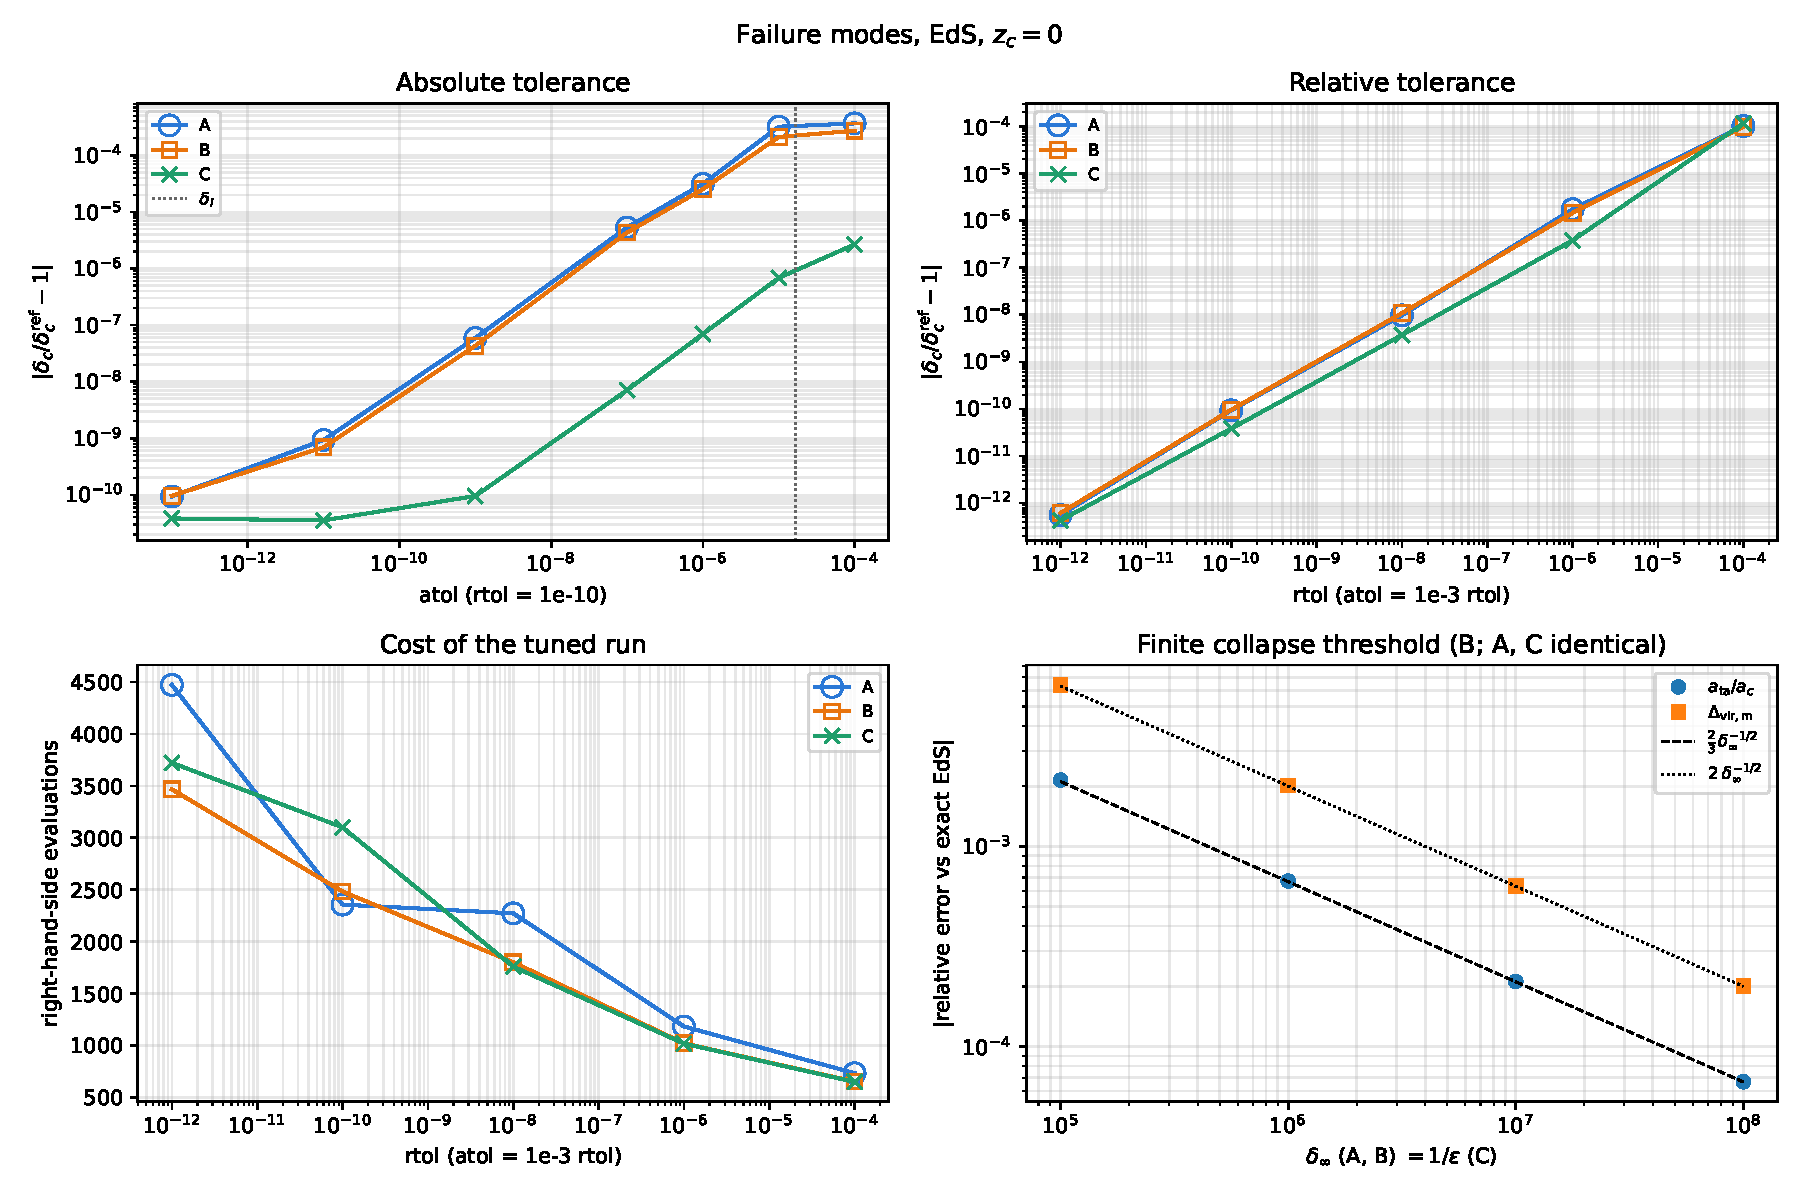
\includegraphics[width=\textwidth]{figures/failure_modes.pdf}
\caption{Failure modes, EdS, $z_c=0$. Top: error of $\delta_c$ against the tightest run (\texttt{rtol=1e-13}, \texttt{atol=1e-16}) of each formulation, as a function of \texttt{atol} (\texttt{rtol=1e-10}) and \texttt{rtol} (\texttt{atol}$=10^{-3}$\,\texttt{rtol}). Bottom left: cost of the tuned run. Bottom right: errors of $a_{\rm ta}/a_c$ and $\Delta_{{\rm vir},m}$ against the exact EdS values as a function of the threshold (B; A, C identical).}
\label{fig:failure}
\end{figure}

\FloatBarrier
The figure separates the failure modes: A and B lose accuracy when \texttt{atol} approaches the initial amplitude $\delta_i$, while C does not ($g=1/\delta_i$ is large). \texttt{rtol} limits all three equally (error $\approx$ \texttt{rtol}), and A is the most expensive at the tightest tolerance. The threshold produces the same error in all formulations, $\propto\delta_\infty^{-1/2}$ and is the dominant error.

%------------------------------------------------------------------------------------------------
\section{Code and reproduction}

\texttt{scripts/exercise\_4.py}: background and shared integration, shooting (\texttt{tune\_delta\_i}) and turnaround/virial step (\texttt{turnaround\_virial}) in the abstract class \texttt{Background}; formulations \texttt{A}, \texttt{B}, \texttt{C} with their own equations, initial conditions and events; \texttt{virial\_y} for the root of eq.~\eqref{eq:cubic}. The growth rate $f_i$ and the growth factor come from \texttt{Cosmology} in \texttt{scripts/exercise\_1.py}. The notebook \texttt{notebooks/exercise\_4.ipynb} produces all tables and figures and saves them in \texttt{report\_ex4/data} and \texttt{report\_ex4/figures}; see \texttt{report\_ex4/README.md} for dependencies and commands.

\begin{thebibliography}{9}
\bibitem{Pace2017} F.~Pace, S.~Meyer, M.~Bartelmann, ``On the implementation of the spherical collapse model for dark energy models'', JCAP \textbf{10}, 040 (2017), \href{https://arxiv.org/abs/1708.02477}{arXiv:1708.02477}.
\bibitem{Notes} T.~Castro, \emph{Spherical Collapse: from the EdS solution to halo abundances}, Numerical Cosmology Lecture~8 notes.
\end{thebibliography}

\end{document}
